% -*- TeX-master: "main"; fill-column: 72 -*-
\section{Introduction}
\label{introduction}
The Systems Biology Graphical Notation (SBGN) aims to standardize the graphical/visual representation of biochemical and cellular processes \citep{sbgn:2009, Junker2012, Czauderna2017, Toure2018}. The goal of SBGN is to represent networks of biochemical interactions in a standard, unambiguous way to foster efficient and accurate representation, visualization, storage, exchange, and reuse of various types of biological knowledge (e.g., gene regulation, metabolism, and cellular signaling). SBGN is defined by comprehensive sets of symbols with precise semantics, together with detailed syntactic rules defining their use and interpretation. Overall, SBGN is made up of  three complementary visual languages. 

\begin{itemize}
  \item The SBGN Process Description (PD) language \citep{Rougny2019} visualizes the temporal courses of the molecular processes and interactions taking place between biochemical entities in a particular system. This type of diagram depicts how entities transition from one form to another as a result of different influences to describe the temporal aspects of a biological system. Nodes describe entity pools (e.g., metabolites, proteins, and complexes) and processes (e.g., associations and influences). The edges describe relationships between the nodes (e.g., consumption and stimulation).
  \item The SBGN Entity Relationship (ER) language \citep{Sorokin2015} visualizes the relationships in which a given entity can participate without regard for the temporal aspects. Relationships can be seen as rules describing the influences of entity pool nodes on relationships. Relationships are independent, and this independence is essential in avoiding the combinatorial explosion inherent to process description diagrams. The nodes describe biological entities such as proteins and complexes, and the edges between them describe interactions, relationships and/or influences (e.g., complex formation, stimulation, and inhibition). 
  \item The SBGN Activity Flow (AF) language \citep{Mi2015} visualizes the influences between the activities displayed by molecular entities, rather than the entities themselves. Nodes in SBGN AF diagrams describe the biological activities of the entities such as protein kinase activity or binding activity. The edges describe influences between the activities (e.g., positive influence and negative influence).
\end{itemize}
  
Formal specification describing the visual languages of SBGN, as well as other materials and software, are available from the SBGN project web site, \url{http://sbgn.org}. The SBGN project seeks a standardized intermediate format---a \emph{lingua franca}---enabling communication of the essential aspects of the visual representations of networks of biochemical interactions.

SBGN is defined neutrally concerning programming languages and software encoding; however, it is oriented primarily towards allowing models to be encoded using XML, the eXtensible Markup Language~\citep{bray:2004}. This document contains specifications of how SBGN maps should be serialized in XML. Note that this specification is related to all three SBGN languages, with classes such as Glyph and Arc having the same definition and attributes across all languages. Unlike SBGN, SBGNML does not deal with biological meaning, but, instead, focuses on the computational representation of SBGN graphics, so it is comparable with graphical exchange standards like GraphML\footnote{\url{http://graphml.graphdrawing.org/}} and SVG\footnote{\url{https://www.w3.org/Graphics/SVG/}}.

This document describes Milestone 3 (known as Version 0.3) of SBGNML. The previous version of this work (SBGNML Milestone 2) was released in 2011 \citep{Iersel2012}. Below is a list of major changes from previous work:

\begin{itemize}
  \item The ability to store multiple SBGN maps within a single file. An ``id'' attribute has added as an identifier for individual SBGN maps to disambiguate them.
  \item The ``language'' attribute has been deprecated to add a ``version'' attribute. The value for this attribute is a URI identifier that gives metadata information about the SBGN language, level, and version of the map.
  \item Complete support for submaps has been implemented with the inclusion of two attributes: ``mapRef'' and ``tagRef''.
  \item The SBGN AF ``perturbation'' glyph, which was an activity node, has been deprecated and is now a unit of information.
  \item The support of colors and other annotations through extensions enables the storage of rendering information and biological annotations (e.g., database identifiers).
\end{itemize}

The definition of the model description language presented here does not specify \emph{how} programs should communicate or read/write SBGN. We assume that for diagram editing software to communicate a model encoded in SBGN, the program will have to translate its internal data structures to and from SBGNML, use a suitable transmission medium and protocol, and to provide any further necessary infrastructure. However, these issues are outside the scope of this document. The software library libSBGN \citep{Iersel2012} was developed for reading, writing, and manipulating SBGN maps stored in SBGNML format. A broad set of software tools support SBGNML, including modeling software CellDesigner \citep{Balaur2020}, SBGN editors Newt \citep{Sari2015}, Krayon for SBGN\footnote{\url{https://github.com/draeger-lab/krayon4sbgn}}, and SBGN-ED \citep{Czauderna2010}. STON \citep{Toure2016} and ySBGN\footnote{\url{https://github.com/sbgn/ySBGN}} provide conversion between SBNGML and GraphML/Neo4j, respectively. The software EscherConverter provides an SBGN viewer and a bidirectional converter for metabolic maps in JSON format and SBGNML \citep{King2015a}. Numerous databases (Reactome \citep{Croft2011}, Panther Pathways \citep{Mi2017}, Pathways Commons \citep{Rodchenkov2020}, PathWhiz \citep{Pon2015}, Path2Models \citep{Buechel2013b}, MetaCrop \citep{Schreiber2012} and Atlas of Cancer Signaling Networks \citep{Kuperstein2015}) provide SBGNML export.

\section{Package syntax and semantics}


\subsection{Document conventions} \label{conventions} 

We use Unified Modeling Language (UML) version 2.0 (\citealt{dennis:2015}) class diagram notation to 
define the constructs provided by this package. We first provide an overall view of the various data types and constructs along with their relationships, followed by a more local view of the constructs and their relationships in associated sections. 

In this section, we define the syntax and semantics of the
\SystemsBiologyGraphicalNotationMarkupLanguagePackage. We expound on the various data types and constructs
defined in this package, then in \sec{examples}; we provide complete
examples of using the constructs in sample SBGN models.

\subsection{Namespace URI and other declarations necessary for using this package}
\label{xml-namespace}

SBGNML is identified uniquely by an XML namespace URI. An SBGN document must declare the following is the namespace URI for this version of the
\SystemsBiologyGraphicalNotationMarkupLanguagePackage for SBGNML version~0.3:

\begin{center}
\uri{http://sbgn.org/libsbgn/0.3}
\end{center}

\begin{figure}[ht!]
  \centering
  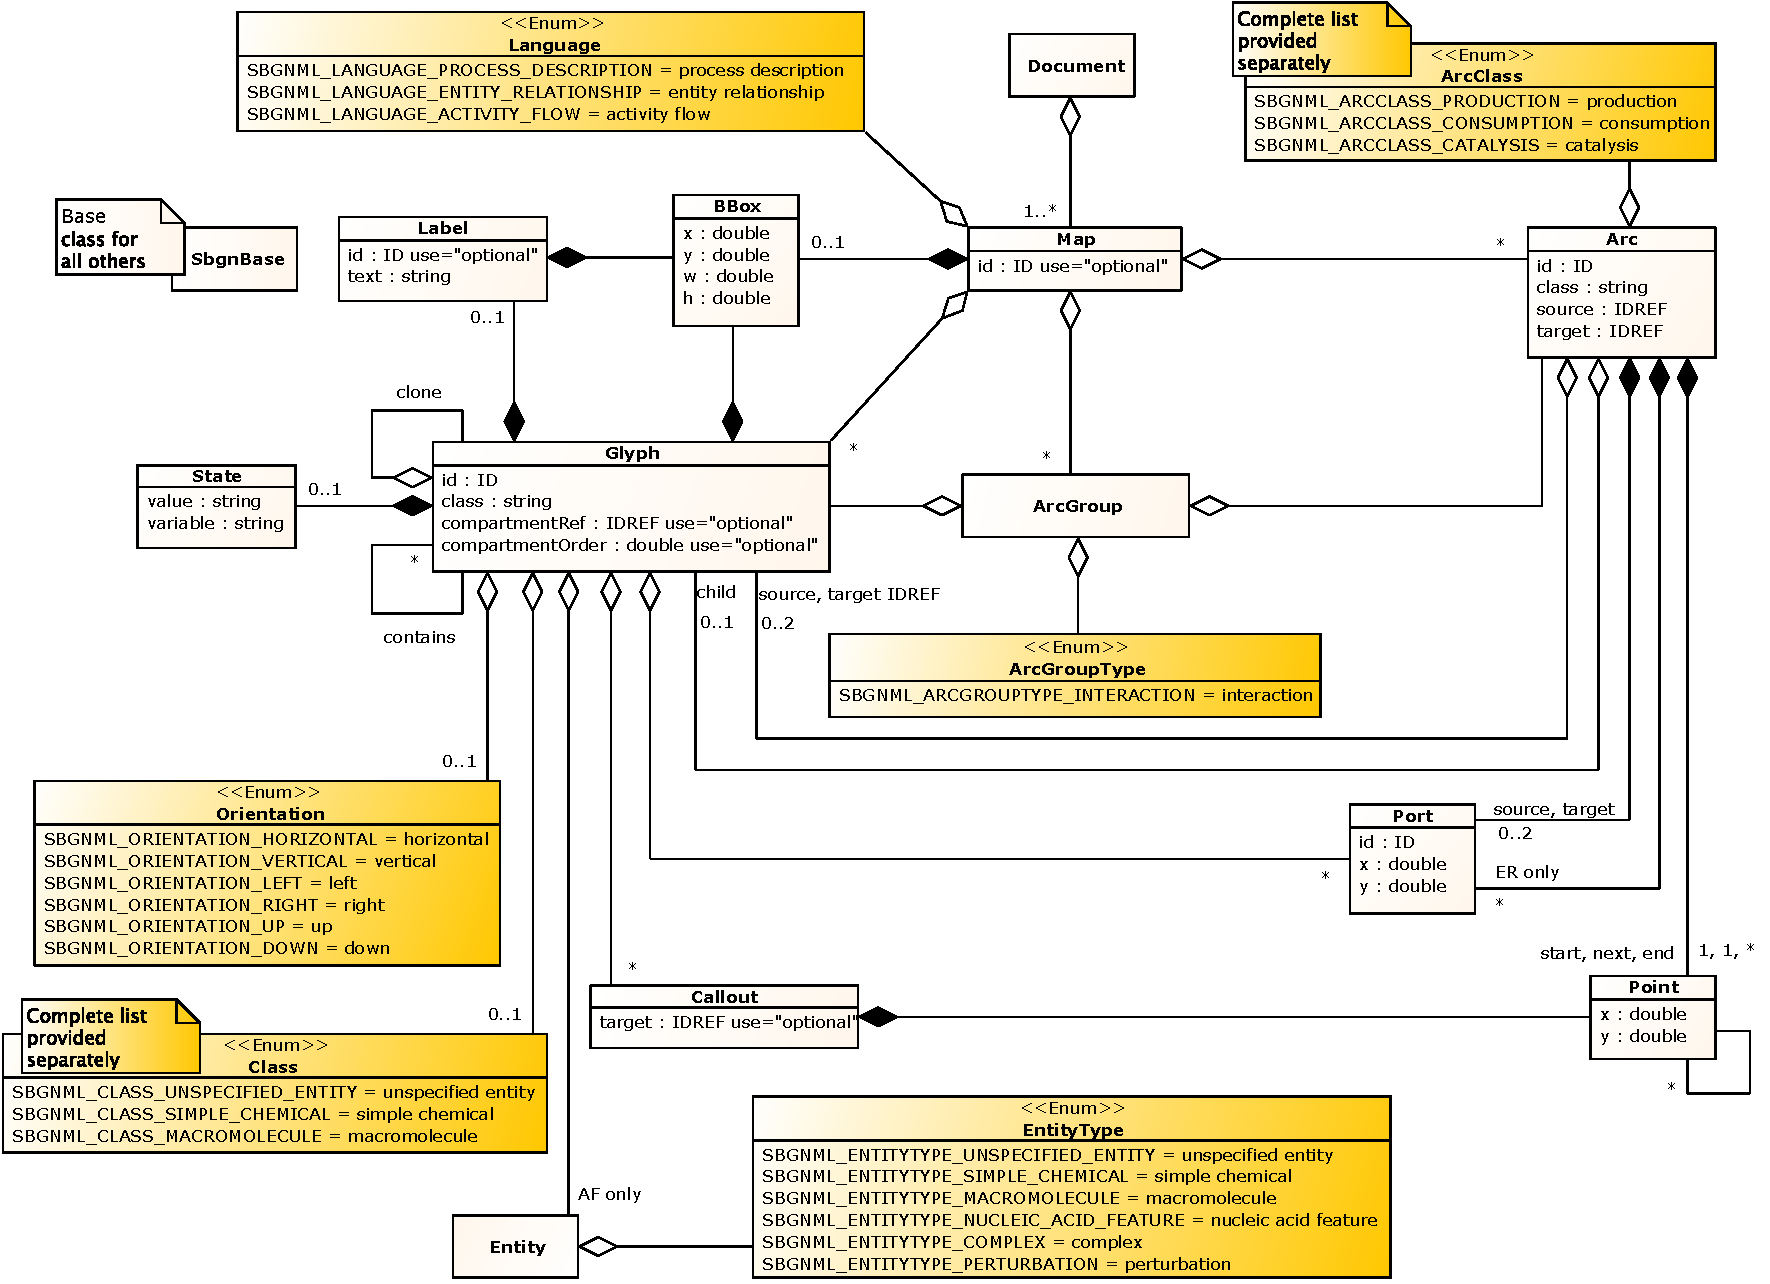
\includegraphics[width=\textwidth]{figures/sbgnml_version_0_complete.pdf}\\
\caption{A UML representation of the \SbgnmlPackage. See
\ref{conventions} for conventions related to this figure. }
  \label{fig:sbgnml_version_0_complete}
\end{figure}

\subsection{Primitive data types}
\label{primitive-types}

Section~3.1 of the SBML Level~3 specification \citep{Hucka2019} defines several
primitive data types and also uses XML Schema 1.0 data types
\citep{biron:2000}. We assume and use some of them in the rest of this
specification, particularly \primtype{float}, \primtype{ID},
\primtype{IDREF}, and \primtype{string}. The
\SystemsBiologyGraphicalNotationMarkupLanguagePackage defines other
primitive types as described below.

\subsubsection{Type \fixttspace\primtypeNC{Language}}

\begin{figure}[ht!]
  \centering
  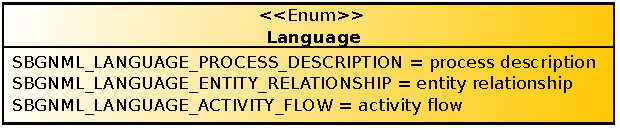
\includegraphics[scale=0.7]{figures/sbgnml_type_enum_language_uml.pdf}\\
\caption{A UML representation of the \Language type for the
\SbgnmlPackage. See \ref{conventions} for conventions related to this
figure. }
  \label{fig:sbgnml_type_enum_language_uml}
\end{figure}


The \primtype{Language} is an enumeration of values used to specify which SBGN Language is encoded on the \Map element.

The possible values are \const{process description}, \const{entity relationship}, and \const{activity flow}.

\subsubsection{Type \fixttspace\primtypeNC{Class}}

\begin{figure}[ht!]
  \centering
  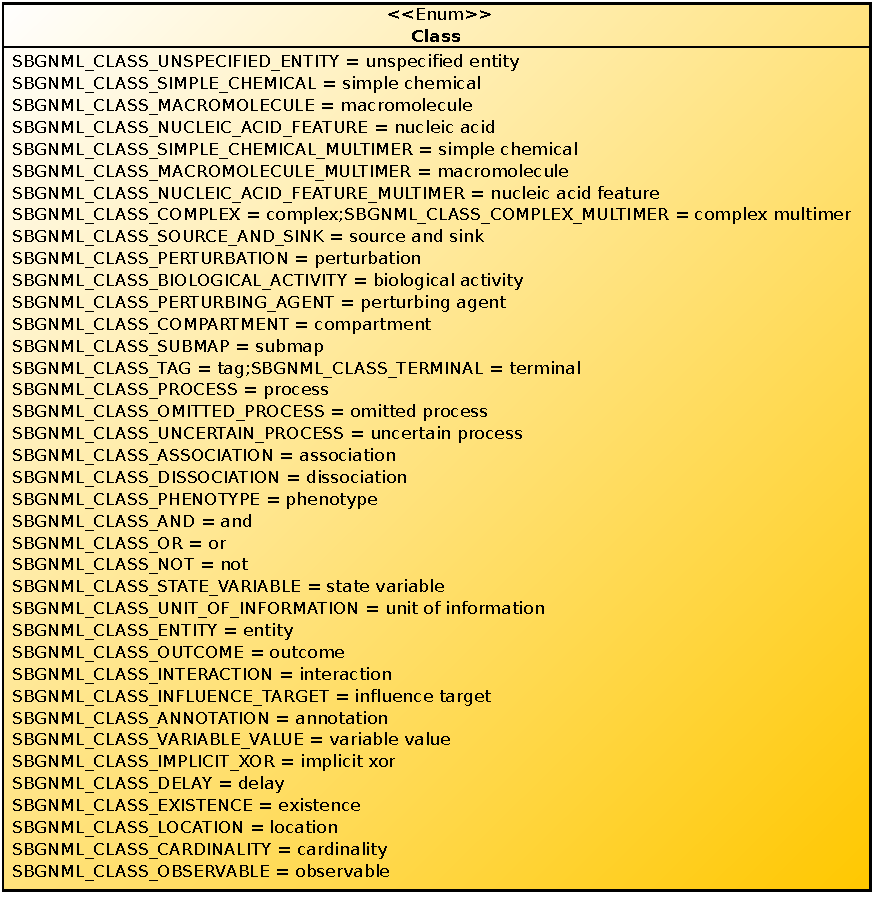
\includegraphics[scale=0.7]{figures/sbgnml_type_enum_class_uml.pdf}\\
\caption{A UML representation of the \Class type for the \SbgnmlPackage.
See \ref{conventions} for conventions related to this figure. }
  \label{fig:sbgnml_type_enum_class_uml}
\end{figure}


The \primtype{Class} is an enumeration of values used to specify what type a \Glyph is encoding. 

The possible values are \const{unspecified entity}, \const{simple
chemical}, \const{macromolecule}, \const{nucleic acid feature},
\const{simple chemical multimer}, \const{macromolecule multimer},
\const{nucleic acid feature multimer}, \const{complex}, \\ \const{complex multimer}, \const{source and sink}, \const{perturbation},
\const{biological activity}, \const{perturbing agent}, \\
\const{compartment}, \const{submap}, \const{tag}, \const{terminal},
\const{process}, \const{omitted process}, \const{uncertain process},
\const{association}, \const{dissociation}, \const{phenotype},
\const{and}, \const{or}, \const{not}, \const{equivalence}, \const{state variable},
\const{unit of information}, \const{entity}, \const{outcome},
\const{interaction}, \const{influence target}, \const{annotation},
\const{variable value}, \const{implicit xor}, \const{delay}, \\ \const{existence}, \const{location}, \const{cardinality}, and
\const{observable}.

\subsubsection{Type \fixttspace\primtypeNC{Orientation}}

\begin{figure}[ht!]
  \centering
  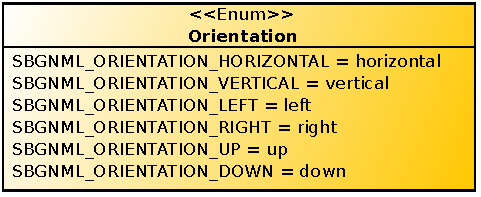
\includegraphics[scale=0.7]{figures/sbgnml_type_enum_orientation_uml.pdf}\\
\caption{A UML representation of the \Orientation type for the
\SbgnmlPackage. See \ref{conventions} for conventions related to this
figure. }
  \label{fig:sbgnml_type_enum_orientation_uml}
\end{figure}


The \primtype{Orientation} is an enumeration of values used to express how to draw asymmetric glyphs. 

The orientation of Process Nodes is either ``horizontal'' or ``vertical''. It refers to an (imaginary) line connecting the two in/out sides of the PN.

The possible values are \const{horizontal}, \const{vertical},
\const{left}, \const{right}, \const{up}, and \const{down}.
The value refers to the direction at which the arrow side of the glyph is pointing.



\subsubsection{Type \fixttspace\primtypeNC{EntityType}}

\begin{figure}[ht!]
  \centering
  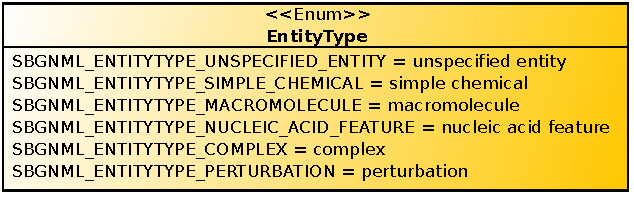
\includegraphics[scale=0.7]{figures/sbgnml_type_enum_entitytype_uml.pdf}\\
\caption{A UML representation of the \EntityType type for the
\SbgnmlPackage. See \ref{conventions} for conventions related to this
figure. }
  \label{fig:sbgnml_type_enum_entitytype_uml}
\end{figure}


The \primtype{EntityType} is an enumeration of values used for Activity Flow maps 
that specifies the auxiliary unit to display. 

The possible values are \const{unspecified entity}, \const{simple
chemical}, \const{macromolecule}, \const{nucleic acid feature}, and
\const{complex}.

\subsubsection{Type \fixttspace\primtypeNC{ArcGroupType}}

\begin{figure}[ht!]
  \centering
  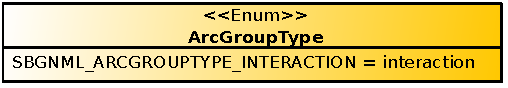
\includegraphics[scale=0.7]{figures/sbgnml_type_enum_arcgrouptype_uml.pdf}\\
\caption{A UML representation of the \ArcGroupType type for the
\SbgnmlPackage. See \ref{conventions} for conventions related to this
figure. }
  \label{fig:sbgnml_type_enum_arcgrouptype_uml}
\end{figure}


The \primtype{ArcGroupType} is an enumeration of values used to define the semantic of an \ArcGroup. 

The only possible value is \const{interaction}.

\subsubsection{Type \fixttspace\primtypeNC{ArcClass}}

\begin{figure}[ht!]
  \centering
  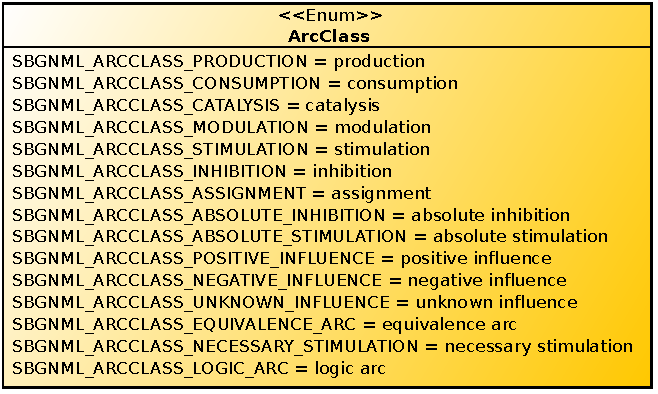
\includegraphics[scale=0.7]{figures/sbgnml_type_enum_arcclass_uml.pdf}\\
\caption{A UML representation of the \ArcClass type for the
\SbgnmlPackage. See \ref{conventions} for conventions related to this
figure. }
  \label{fig:sbgnml_type_enum_arcclass_uml}
\end{figure}


The \primtype{ArcClass} is an enumeration of values used to define the semantic of an \Arc. 


The possible values are \const{production}, \const{consumption},
\const{catalysis}, \const{modulation}, \const{stimulation},
\const{inhibition}, \const{assignment}, \const{absolute inhibition},
\const{absolute stimulation}, \const{positive influence},
\const{negative influence}, \const{unknown influence},
\const{equivalence arc}, \const{necessary stimulation}, and \const{logic
arc}.

% ---------------------------------------------------------
\subsection{The \class{SBGN} class}
\label{document-class}

\begin{figure}[ht!]
  \centering
  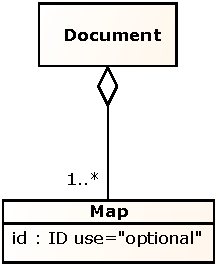
\includegraphics[scale=1.0]{figures/sbgnml_document_uml.pdf}\\
\caption{A UML representation of the \Document class for the
\SbgnmlPackage. See \ref{conventions} for conventions related to this
figure. }
  \label{fig:sbgnml_document_uml}
\end{figure}

The \Document object shown in \ref{fig:sbgnml_document_uml} corresponds to the XML element \token{sbgn}.
The \token{sbgn} element is the root of any SBGNML document.


The \Document object derives from the \SbgnBase class and thus inherits all attributes and elements that are present for this class.
A \Document contains one or more \Map elements.

\paragraph{Example}

The following example shows an \token{sbgn} element definition. 

\begin{example}
<sbgn ...>
    ...
</sbgn>\end{example}


% ---------------------------------------------------------
\subsection{The \class{Map} class}
\label{map-class}

\begin{figure}[ht!]
  \centering
  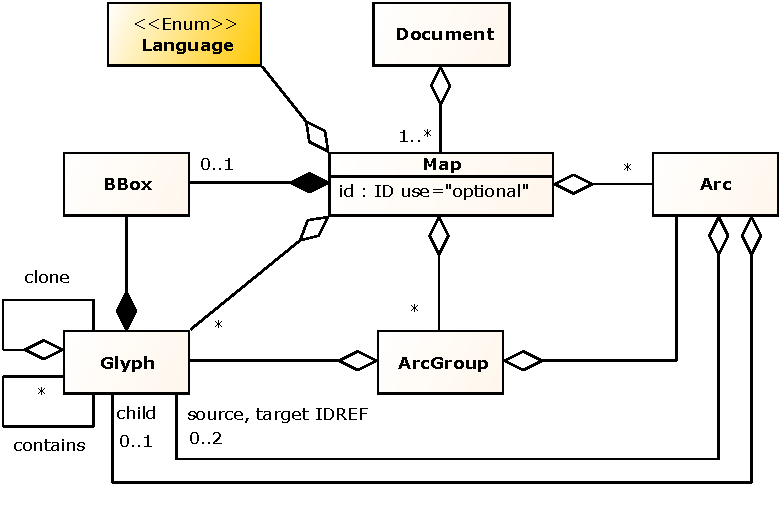
\includegraphics[scale=1.0]{figures/sbgnml_map_uml.pdf}\\
\caption{A UML representation of the \Map class for the \SbgnmlPackage.
See \ref{conventions} for conventions related to this figure. }
  \label{fig:sbgnml_map_uml}
\end{figure}


The \token{map} element describes a single SBGN map.

The \Map object derives from the \SbgnBase class and thus inherits all
attributes and elements that are present for this class.
A \Map contains exactly one \BBox element.

A \Map may contain one or more:

\begin{itemize}
  \item \Glyph elements.
  \item \Arc elements.
  \item \ArcGroup elements.
\end{itemize}

In addition, the \Map object has the following attributes.

\paragraph{The \fixttspace\token{id} attribute}

A \Map has an optional attribute \token{id} of type \primtype{ID}.


\paragraph{The \fixttspace\token{language} attribute}

A \Map has an optional attribute \token{language} of type
string. While the type is of \primtype{string}, the values should be one of the ones defined in \primtype{Language}, i.e., one of the following:

\begin{itemize}
	\item \token{process description}
  \item \token{entity relationship}
  \item \token{activity flow}
\end{itemize}

The \token{language} attribute has been deprecated as of Version~0.3, in favor of the \token{version} attribute. One of the attributes has to be defined on a map element.

\paragraph{The \fixttspace\token{version} attribute}

A \Map has an optional attribute \token{version} of type
\primtype{URI} with the URL to the SBGN language and version it is referring to. The attribute can take one of the following values:

\begin{itemize}
  \item \url{http://identifiers.org/combine.specifications/sbgn.pd.level-1.version-2.0}
  \item \url{http://identifiers.org/combine.specifications/sbgn.pd.level-1.version-1.3}
  \item \url{http://identifiers.org/combine.specifications/sbgn.pd.level-1.version-1.2}
  \item \url{http://identifiers.org/combine.specifications/sbgn.pd.level-1.version-1.1}
  \item \url{http://identifiers.org/combine.specifications/sbgn.pd.level-1.version-1.0}
  \item \url{http://identifiers.org/combine.specifications/sbgn.pd.level-1.version-1}
  \item \url{http://identifiers.org/combine.specifications/sbgn.er.level-1.version-2}
  \item \url{http://identifiers.org/combine.specifications/sbgn.er.level-1.version-1.2}
  \item \url{http://identifiers.org/combine.specifications/sbgn.er.level-1.version-1.1}
  \item \url{http://identifiers.org/combine.specifications/sbgn.er.level-1.version-1.0}
  \item \url{http://identifiers.org/combine.specifications/sbgn.er.level-1.version-1}
  \item \url{http://identifiers.org/combine.specifications/sbgn.af.level-1.version-1.2}
  \item \url{http://identifiers.org/combine.specifications/sbgn.af.level-1.version-1.0}
  \item \url{http://identifiers.org/combine.specifications/sbgn.af.level-1.version-1}
\end{itemize}

The \token{version} attribute should be used in favor of the \token{language} attribute. One of the attributes has to be defined on a map element.

\paragraph{Example}

The following example shows an abbreviated SBGN \Map definition within an sbgn element definition. The example shows a \Map with a \token{version} attribute.

\begin{example}
<sbgn ...>
    ...
    <map id="m1" version="http://identifiers.org/combine.specifications/sbgn.pd.level-1.version-1.3">
        ...
    </map>
    ...
</sbgn>
\end{example}


% ---------------------------------------------------------
\subsection{The \class{Point} class}
\label{point-class}

\begin{figure}[ht!]
  \centering
  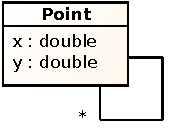
\includegraphics[scale=1.0]{figures/sbgnml_point_uml.pdf}\\
\caption{A UML representation of the \Point class for the
\SbgnmlPackage. See \ref{conventions} for conventions related to this
figure. }
  \label{fig:sbgnml_point_uml}
\end{figure}


The \Point object encodes \token{x} and \token{y} coordinates. 

The origin is located in the top-left corner of the map.

There is no unit: proportions must be preserved, but the maps can be drawn at any scale. In the example test files, to obtain a drawing similar to the reference \value{*.png} file, values in the corresponding \value{*.sbgn} file should be read as pixels.

Additionally, it may contain zero, one, or two child \Point objects, which can be used to encode quadratic or cubic B\'{e}zier points. 

The \Point object derives from the \SbgnBase class and thus inherits all
attributes and elements that are present for this class.
In addition, the \Point object has the following attributes.

\paragraph{The \fixttspace\token{x} attribute}

A \Point has a required attribute \token{x} of type \primtype{double}. It represents the Cartesian \token{x} coordinate horizontally, increasing from left to right.


\paragraph{The \fixttspace\token{y} attribute}

A \Point has a required attribute \token{y} of type \primtype{double}. It represents the Cartesian \token{y} coordinate vertically, increasing from top to bottom.

\paragraph{Example}

The following example shows a \Point definition within an abbreviated SBGN map definition. The example shows a \Point on a \Callout.

\begin{example}
<map ...>
    ...
    <glyph ...>
        ...
        <callout ...>
            <point x="100.0" y="200.0"/>
        </callout>
        ...
    </glyph>
    ...
</map>
\end{example}


% ---------------------------------------------------------
\subsection{The \class{BBox} class}
\label{bbox-class}

\begin{figure}[ht!]
  \centering
  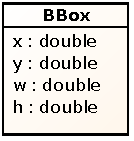
\includegraphics[scale=1.0]{figures/sbgnml_bbox_uml.pdf}\\
\caption{A UML representation of the \BBox class for the \SbgnmlPackage.
See \ref{conventions} for conventions related to this figure. }
  \label{fig:sbgnml_bbox_uml}
\end{figure}


\BBox encodes the bounding box of its parent element. 

The \BBox object derives from the \SbgnBase class and thus inherits all
attributes and elements that are present for this class.
In addition, the \BBox object has the following attributes.

\paragraph{The \fixttspace\token{x} attribute}

A \BBox has a required attribute \token{x} of type \primtype{double}. It represents the Cartesian \token{x} coordinate horizontally, increasing from left to right.


\paragraph{The \fixttspace\token{y} attribute}

A \BBox has a required attribute \token{y} of type \primtype{double}. It represents the Cartesian \token{y} coordinate vertically, increasing from top to bottom.


\paragraph{The \fixttspace\token{w} attribute}

A \BBox has a required attribute \token{w} of type
\primtype{double}. It encodes the width of the bounding box. 


\paragraph{The \fixttspace\token{h} attribute}

A \BBox has a required attribute \token{h} of type
\primtype{double}. It encodes the height of the bounding box. 

\paragraph{Example}

The following example shows a \BBox definition within an abbreviated SBGN map definition. The example shows the \BBox on a \Glyph.

\begin{example}
<map ...>
    ...
    <glyph ...>
        ...
        <bbox x="10.0" y="10.0" w="100.0" h="50.0"/>
        ...
    </glyph>
    ...
</map>
\end{example}


% ---------------------------------------------------------
\subsection{The \class{Label} class}
\label{label-class}

\begin{figure}[ht!]
  \centering
  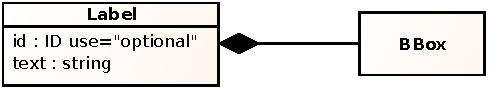
\includegraphics[scale=1.0]{figures/sbgnml_label_uml.pdf}\\
\caption{A UML representation of the \Label class for the
\SbgnmlPackage. See \ref{conventions} for conventions related to this
figure. }
  \label{fig:sbgnml_label_uml}
\end{figure}


The \Label element describes the text accompanying a glyph.

The \Label object derives from the \SbgnBase class and thus inherits all
attributes and elements that are present for this class.
A \Label may contain exactly one \BBox element.
In addition, the \Label object has the following attributes.

\paragraph{The \fixttspace\token{id} attribute}

A \Label has an optional attribute \token{id} of type \primtype{ID}.


\paragraph{The \fixttspace\token{text} attribute}

A \Label has a required attribute \token{text} of type
\primtype{string}. The text element is a simple string. Multi-line labels are allowed. Line breaks are encoded as \token{\&\#xA;} as specified by the XML standard.

\paragraph{The \BBox element of a \Label}

The \token{bbox} element of a label is optional. When no bounding box is defined, the bounding box of the parent glyph is inherited. The label should be drawn centered horizontally and vertically in the bounding box.

When the bounding box is inherited, the label may spill outside (just like it can spill outside its parent glyph).

An explicit \token{bbox} provides more definite information regarding what surface the label should cover. It defines an upper boundary outside of which the label should (ideally) not spill. It also represents a preferred size: the surface covered by the label can be smaller, but should ideally be as close as possible to the bounding box.

In most glyph classes (EPNs, unit of information, etc.), the label is supposed to be centered, so the bounding box is usually omitted (unless there is a specific hint to be shared concerning the area the label should ideally cover).

However, the label of a compartment or a complex can be drawn anywhere inside the glyph, so these should preferably have an explicit bounding box.

\paragraph{Example}

The following example shows a \Label definition within an abbreviated SBGN map definition. The example shows the \Label without a \token{bbox} element on a \Glyph.

\begin{example}
<map ...>
    ...
    <glyph ...>
        ...
        <label text="label"/>
        ...
    </glyph>
    ...
</map>
\end{example}


% ---------------------------------------------------------
\subsection{The \class{Glyph} class}
\label{glyph-class}

\begin{figure}[ht!]
  \centering
  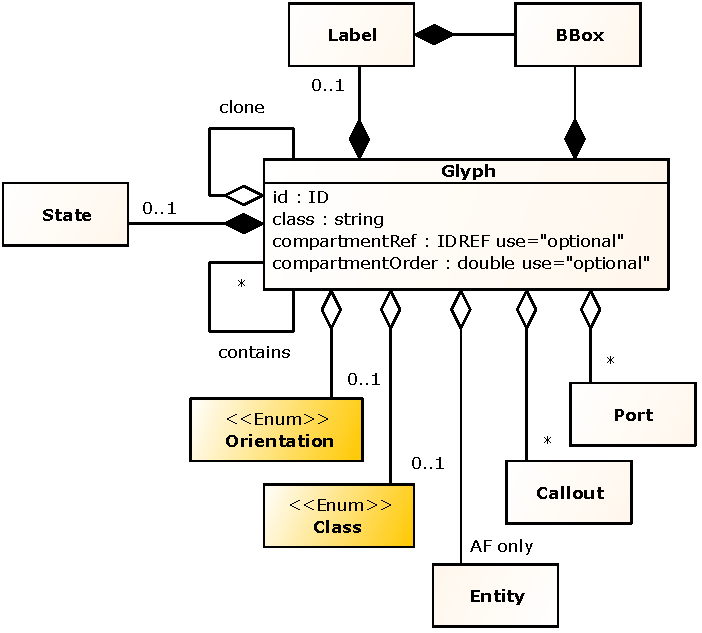
\includegraphics[scale=1.0]{figures/sbgnml_glyph_uml.pdf}\\
\caption{A UML representation of the \Glyph class for the
\SbgnmlPackage. See \ref{conventions} for conventions related to this
figure. }
  \label{fig:sbgnml_glyph_uml}
\end{figure}


The glyph element is:

\begin{itemize}
	\item {either a stand-alone, high-level SBGN node (an EPN, PN, compartment, etc.)}
\item {or a sub-node (state variable, unit of information, inside of a complex, etc.)}

\end{itemize}

In the first case, it is a child of the map element.

In the second case, it is a child of another glyph element.

The \Glyph object derives from the \SbgnBase class and thus inherits all
attributes and elements that are present for this class.

A \Glyph contains: 

\begin{itemize}
  \item exactly one \BBox element that describes the bounding box of the glyph.
\end{itemize}

A \Glyph may contain: 

\begin{itemize}
  \item exactly one \Label element that describes the text accompanying the glyph.
  \item exactly one \State element that carries the information of a state variable.
  \item exactly one \Glyph element called ``clone'', indicating that the Glyph carries a clone marker. The label element of the child glyph can be used to place text in the clone marker. \ref{fig:glyph_clone_example} shows an example. 
  \item exactly one \Callout element. The callout element is only used for glyphs of class \const{annotation}. It contains the coordinate of the point where the annotation points to, as well as a reference to the element that is pointed to.
  \item exactly one \Entity element. The entity is only used in Activity Flow maps. It can only be used on a unit of information glyph on a biological activity glyph, where it is compulsory. It is used to indicate the shape of this unit of information.
  %\item exactly one \Entity element. The entity is only used in Activity Flow maps. It can only be used on a unit of information glyph on a biological activity glyph, where it is compulsory. It is used to indicate the shape of this unit of information.
  \item zero or more child \Glyph elements. These will be, for example, used by glyphs of class \const{complex} and hold the individual components.
  \item zero or more child \Port elements describing the anchor points for this glyph.
\end{itemize}

%A \Glyph contains: 

%\begin{itemize}
%  \item exactly one \Glyph element called ``clone'', when it is set, it indicates that the Glyph carries a clone marker. The label element of the child glyph can be used to  place text in the clone marker.
%  \item exactly one \BBox element that describes the bounding box of the glyph.
%\end{itemize}

%A \Glyph can contain: 

%\begin{itemize}
%  \item zero or more child \Glyph elements. This will be for example used by glyphs of class \const{complex} and hold the individual components.
%  \item zero or more child \Port elements describing the anchor points for this glyph.
%\end{itemize}

In addition, the \Glyph object has the following attributes.

\paragraph{The \fixttspace\token{id} attribute}

A \Glyph has a required attribute \token{id} of type \primtype{ID}. The \token{id} attribute (\token{xsd:ID}) of a glyph can be referred to, e.g.,  as a source by arc elements, a target by arc elements or callout elements, by other glyphs if the glyph is of the class \const{compartment}.

The \token{xsd:ID} type is an alphanumeric identifier, starting with a letter.

It is recommended to generate meaningless IDs (e.g., ``\token{glyph1234}'') and avoid IDs with meaning (e.g., ``\token{epn\_ethanol}'')


\paragraph{The \fixttspace\token{class} attribute}

A \Glyph has a required attribute \token{class} of type
\primtype{string}. While the type is of \primtype{string}, the values should be one of the ones defined in \primtype{Class}.

\paragraph{The \fixttspace\token{compartmentRef} attribute}

A \Glyph has an optional attribute \token{compartmentRef} of type
\primtype{IDREF}.

The \token{compartmentRef} is a reference to the ID of the compartment that this glyph is part of. It should only be used if there is at least one explicit compartment present on the map. Compartments are only used in PD and AF, and thus this attribute as well. For PD, this should be used only for EPNs.

In case there are no compartments, entities that can have a location, such as EPNs, are implicit members of an invisible compartment that encompasses the whole map. In that case, this attribute must be omitted.

\paragraph{The \fixttspace\token{compartmentOrder} attribute}

A \Glyph has an optional attribute \token{compartmentOrder} of type
\primtype{double}.

The \token{compartmentOrder} attribute can be used to define a drawing order for compartments. It enables tools to draw compartments in the correct order, especially in the case of overlapping compartments. Compartments are only used in PD and AF, and, thus, this attribute as well.

The attribute is of type \token{float}, and the attribute value has not to be unique.


Compartments with higher \token{compartmentOrder} are drawn on top. The attribute is optional and should only be used for compartments.

\paragraph{The \fixttspace\token{orientation} attribute}

A \Glyph has an optional attribute \token{orientation} of type string. While the type is of \primtype{string}, the values should be one of the ones defined in \primtype{Orientation}. The \token{orientation} attribute is used to express how to draw asymmetric glyphs.

The orientation of Process Nodes is either \token{horizontal} or \token{vertical}. It refers to an (imaginary) line connecting the two in/out sides of the PN.

The orientation of Tags can be \token{left}, \token{right}, \token{up}, or \token{down}. It refers to the direction at which the arrow side of the glyph is pointing.

\paragraph{Example}

The following example shows a \Glyph definition within an abbreviated SBGN map definition. The example shows a \Glyph of class \const{macromolecule} with an optional attribute \token{compartmentRef}. \ref{fig:glyph_example} shows the corresponding visual representation.

\begin{example}
<map ...>
    ...
    <glyph id="glyph1" class="macromolecule" compartmentRef="glyphcomp1">
        <label text="Glucose"/>
        <bbox x="10.0" y="10.0" w="100.0" h="50.0"/>
    </glyph>
    ...
</map>
\end{example}

\begin{figure}[!ht]
  \centering
  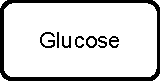
\includegraphics[scale=0.9]{figures/glyph_example.pdf}
\caption{Visual representation of a \Glyph of the class \const{macromolecule}.}
  \label{fig:glyph_example}
\end{figure}

\paragraph{Example Clone Marker}

The following example shows a \Glyph definition within an abbreviated SBGN map definition. The example shows a \Glyph of class \const{macromolecule} with an optional attribute \token{compartmentRef} and a clone marker. \ref{fig:glyph_clone_example} shows the corresponding visual representation.

\begin{example}
<map ...>
    ...
    <glyph id="glyph1" class="macromolecule" compartmentRef="glyphcomp1">
        <clone>
            <label text="marker">
                <bbox x="10.0" y="47.5" w="100.0" h="12.5"/>
            </label>
        </clone>
        <label text="Glucose"/>
        <bbox x="10.0" y="10.0" w="100.0" h="50.0"/>
    </glyph>
    ...
</map>
\end{example}

\begin{figure}[!ht]
  \centering
  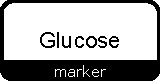
\includegraphics[scale=0.9]{figures/glyph_clone_example.pdf}
\caption{Visual representation of a \Glyph of the class \const{macromolecule} with a clone marker.}
  \label{fig:glyph_clone_example}
\end{figure}



% ---------------------------------------------------------
\subsection{The \class{Port} class}
\label{port-class}

\begin{figure}[ht!]
  \centering
  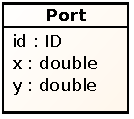
\includegraphics[scale=1.0]{figures/sbgnml_port_uml.pdf}\\
\caption{A UML representation of the \Port class for the \SbgnmlPackage.
See \ref{conventions} for conventions related to this figure. }
  \label{fig:sbgnml_port_uml}
\end{figure}

A port element describes an anchor point, which arc elements can refer to as a source or target. It consists of absolute 2D Cartesian coordinates and a unique id attribute.

Two port elements are required for process nodes and logical operators (\const{and}, \const{or}, \const{not}, and \const{equivalence}). They represent the extremity of the two ``arms'' which protrude on both sides of the core of the glyph (= square or circle shape).

The \Port object derives from the \SbgnBase class and, thus, inherits all
attributes and elements that are present for this class.
In addition, the \Port object has the following attributes.

\paragraph{The \fixttspace\token{id} attribute}

A \Port has a required attribute \token{id} of type \primtype{ID}.


\paragraph{The \fixttspace\token{x} attribute}

A \Point has a required attribute \token{x} of type \primtype{double}. It represents the Cartesian \token{x} coordinate horizontally, increasing from left to right.


\paragraph{The \fixttspace\token{y} attribute}

A \Point has a required attribute \token{y} of type \primtype{double}. It represents the Cartesian \token{y} coordinate vertically, increasing from top to bottom.

\paragraph{Example}

The following example shows a \Port definition within an abbreviated SBGN map definition. The example shows two \Port{}s on a \Glyph.

\begin{example}
<map ...>
    ...
    <glyph id="glyph1" ...>
        ...
        <port id="glyph1.1" x="100.0" y="100.0"/>
        <port id="glyph1.2" x="120.0" y="100.0"/>
        ...
    </glyph>
    ...
</map>
\end{example}


% ---------------------------------------------------------
\subsection{The \class{State} class}
\label{state-class}

\begin{figure}[ht!]
  \centering
  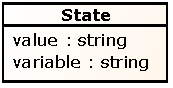
\includegraphics[scale=1.0]{figures/sbgnml_state_uml.pdf}\\
\caption{A UML representation of the \State class for the
\SbgnmlPackage. See \ref{conventions} for conventions related to this
figure. }
  \label{fig:sbgnml_state_uml}
\end{figure}

The state element should only be used for state variables. It replaces the label element used for other glyphs. It describes the text to be drawn inside the state variable.

The \State object derives from the \SbgnBase class and thus inherits all
attributes and elements that are present for this class.
In addition, the \State object has the following attributes.

\paragraph{The \fixttspace\token{variable} attribute}

A \State has an optional attribute \token{variable} of type
\primtype{string}.
It describes the site where the modification described by the value attribute occurs. It is:

\begin{itemize}
	\item optional when there is only one state variable on the parent EPN
  \item required when there is more than one state variable on the parent EPN
\end{itemize}

\paragraph{The \fixttspace\token{value} attribute}

A \State has an optional attribute \token{value} of type
\primtype{string}. It represents the state of the variable. It can be:

\begin{itemize}
	\item either from a predefined set of strings (e.g., ``P'', ``S'', etc.) which correspond to specific SBO terms (cf. SBGN specifications)
\item or any arbitrary \primtype{string}.

\end{itemize}

\paragraph{Example}

The following example shows a \State definition within an abbreviated SBGN map definition. The example depicts two \State{}s on a \Glyph of the class \const{macromolecule}, one \State with a \token{value} attribute and a \token{variable} attribute and one \State with a \token{variable} attribute only.
\vref{fig:state_example} shows the corresponding visual representation.

\begin{example}
<map ...>
    ...
    <glyph id="glyph1" class="entity">
        <label text="CaMKII"/>
        <bbox x="10.0" y="20.0" w="140.0" h="50.0"/>
        <glyph id="glyph1a" class="state variable">
            <state variable="T286" value="P"/>
            <bbox x="13.5" y="11.0" w="63.0" h="18.0"/>
        </glyph>
        <glyph id="glyph1b" class="state variable">
            <state variable="T306"/>
            <bbox x="93.5" y="11.0" w="43.0" h="18.0"/>
        </glyph>
    </glyph>
    ...
</map>
\end{example}

\begin{figure}[!ht]
  \centering
  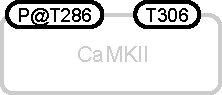
\includegraphics[scale=0.9]{figures/state_example.pdf}
\caption{Visual representation of two \State{}s on a \Glyph of the class \const{macromolecule}.}
  \label{fig:state_example}
\end{figure}


% ---------------------------------------------------------
\subsection{The \class{Callout} class}
\label{callout-class}

\begin{figure}[ht!]
  \centering
  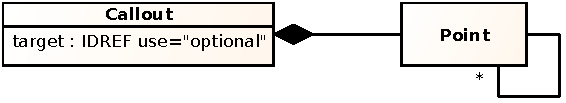
\includegraphics[scale=1.0]{figures/sbgnml_callout_uml.pdf}\\
\caption{A UML representation of the \Callout class for the
\SbgnmlPackage. See \ref{conventions} for conventions related to this
figure. }
  \label{fig:sbgnml_callout_uml}
\end{figure}


Callouts are used in the case of glyphs of class \const{annotation}. The callout is always optional. It can be used to show which element the callout points to.

The \Callout object derives from the \SbgnBase class and thus inherits all
attributes and elements that are present for this class.
A \Callout contains at most one \Point element.
In addition, the \Callout object has the following attributes.

\paragraph{The \fixttspace\token{target} attribute}

A \Callout has an optional attribute \token{target} of type
\primtype{IDREF}. If specified, it references either a \Glyph or an \Arc in the \Map. 

\paragraph{Example}

The following example shows a \Callout definition within an abbreviated SBGN map definition. The example depicts a \Callout on a \Glyph of class \const{annotation}, pointing to a \Glyph of the class \const{macromolecule}. \ref{fig:callout_example} contains the corresponding visual representation.

\begin{example}
<map ...>
    ...
    <glyph id="g1" class="macromolecule">
        <label text="label"/>
        <bbox x="10.0" y="95.0" w="100.0" h="50.0"/>
    </glyph>
    <glyph id="g2" class="annotation">
        <callout target="g1">
            <point x="95.0" y="110.0"/>
        </callout>
        <label text="annotation"/>
        <bbox x="95.0" y="10.0" w="100.0" h="100.0"/>
    </glyph>
    ...
</map>
\end{example}

\begin{figure}[!ht]
  \centering
  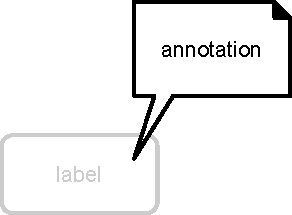
\includegraphics[scale=0.9]{figures/callout_example.pdf}
\caption{Visual representation of a \Callout on a \Glyph of class \const{annotation} pointing to a \Glyph of the class \const{macromolecule}.}
  \label{fig:callout_example}
\end{figure}


% ---------------------------------------------------------
\subsection{The \class{Entity} class}
\label{entity-class}

\begin{figure}[ht!]
  \centering
  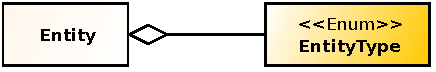
\includegraphics[scale=1.0]{figures/sbgnml_entity_uml.pdf}\\
\caption{A UML representation of the \Entity class for the
\SbgnmlPackage. See \ref{conventions} for conventions related to this
figure. }
  \label{fig:sbgnml_entity_uml}
\end{figure}


An entity is only used in Activity Flow maps. It should be placed on a unit of information subglyph of an activity glyph and is used to indicate the entity that performs the activity.

The \Entity object derives from the \SbgnBase class and thus inherits all
attributes and elements that are present for this class.
In addition, the \Entity object has the following attributes.

\paragraph{The \fixttspace\token{name} attribute}

An \Entity has a required attribute \token{name} of type
\primtype{string}. %An entity is only used in Activity Flow maps. It should be placed on a sub-glyph of an activity glyph, and is used to indicate the entity that performs the activity.

\paragraph{Example}

The following example shows an \Entity definition within an abbreviated SBGN map definition. The example shows an \Entity with the \token{name} ``macromolecule'' placed on a \Glyph of class \const{biological activity}. \ref{fig:entity_example} shows the corresponding visual representation.

\begin{example}
<map ...>
    ...
    <glyph id="glyph1" class="biological activity">
        <label text="Activity"/>
        <bbox x="10.0" y="20.0" w="100.0" h="50.0"/>
        <glyph id="glyph1a" class="unit of information">
            <label text="Entity"/>
            <entity name="macromolecule"/>
            <bbox x="13.0" y="11.0" w="44.0" h="18.0"/>
        </glyph>
    </glyph>
    ...
</map>
\end{example}

\begin{figure}[!ht]
  \centering
  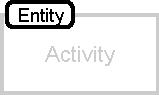
\includegraphics[scale=0.9]{figures/entity_example.pdf}
\caption{Visual representation of an \Entity on a \Glyph of the class \const{biological activity}.}
  \label{fig:entity_example}
\end{figure}


% ---------------------------------------------------------
\subsection{The \class{Arc} class}
\label{arc-class}

\begin{figure}[ht!]
  \centering
  %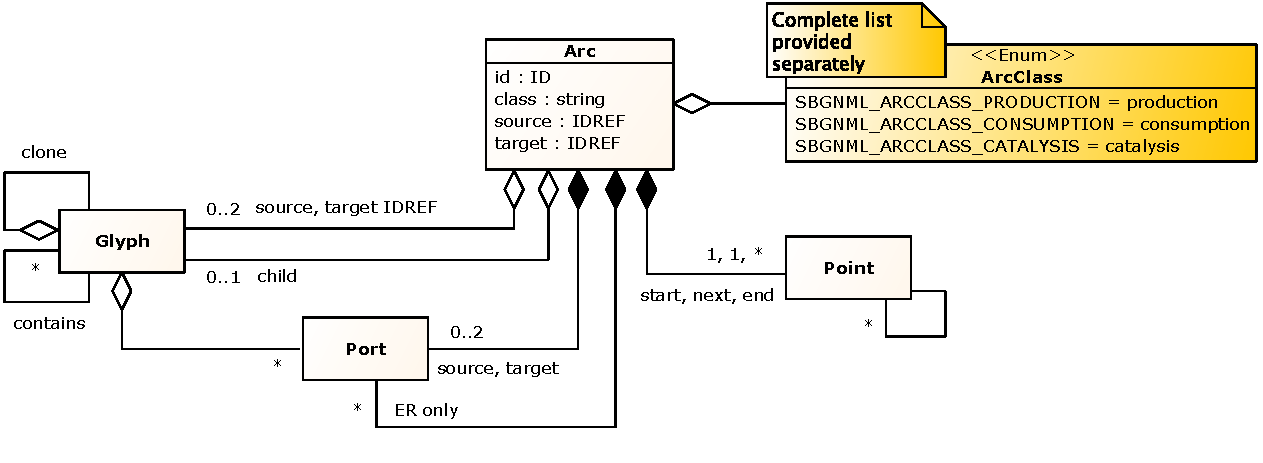
\includegraphics[scale=0.7]{figures/sbgnml_arc_uml.pdf}\\
  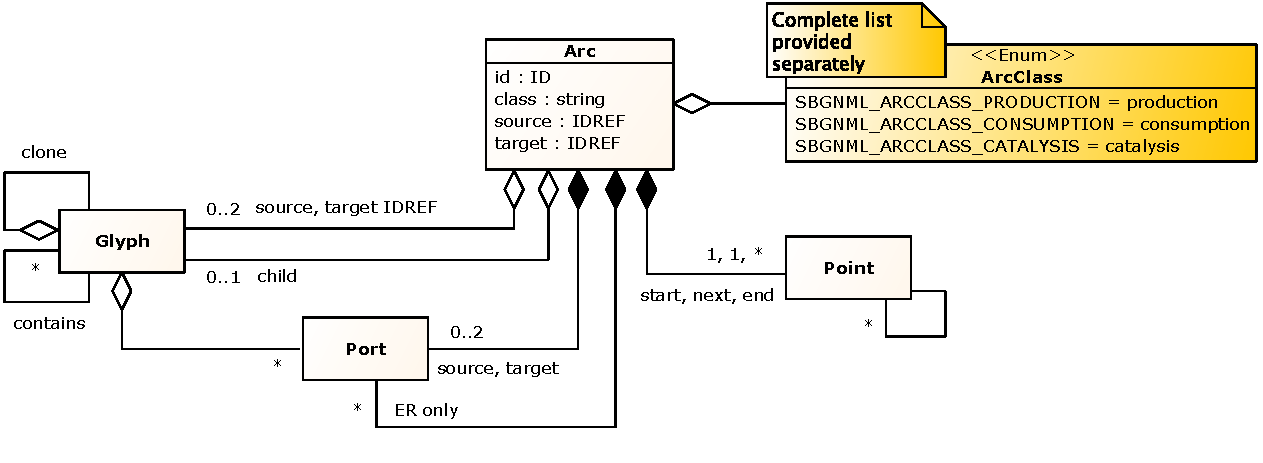
\includegraphics[width=\textwidth]{figures/sbgnml_arc_uml.pdf}\\
\caption{A UML representation of the \Arc class for the \SbgnmlPackage.
See \ref{conventions} for conventions related to this figure. }
  \label{fig:sbgnml_arc_uml}
\end{figure}


The arc element describes an SBGN arc between two SBGN nodes. It contains:

\begin{itemize}
	\item{For PD maps: an optional stoichiometry marker,}

\item {For ER maps: an optional cardinality marker (e.g., ``cis'' or ``trans''), zero or more ports (influence targets), and zero or more outcomes,}
\item {a mandatory source and target (glyph or port),}
\item {a geometric description of its whole path from start to end. This path can involve any number of straight lines or quadratic/cubic B\'{e}zier curves.}

\end{itemize}



The \Arc object derives from the \SbgnBase class and thus inherits all
attributes and elements that are present for this class.

An \Arc can contain zero or more child \Glyph elements. These can be a stoichiometry marker (PD maps), a cardinality marker (ER maps), or outcome glyphs (ER maps). 

An \Arc contains at the very least one \Point element with an element named \token{start} that represents the start point of the arc, and another \Point element with element name \token{end} as the endpoint. Additionally, it may contain any number of \Point elements with element name \token{next} that represent bend points along the way from start to end. 

An \Arc may also contain any number of \Port elements.

In addition, the \Arc object has the following attributes.

\paragraph{The \fixttspace\token{id} attribute}

An \Arc has a required attribute \token{id} of type \primtype{ID}.


\paragraph{The \fixttspace\token{class} attribute}

An \Arc has a required attribute \token{class} of type
\primtype{string}. It describes what kind of an \Arc this element represents. While the data type is of \primtype{string}, the values ought to be from the \primtype{ArcClass} enumeration. 

\paragraph{The \fixttspace\token{source} attribute}

An \Arc has a required attribute \token{source} of type
\primtype{IDREF}. It specifies the source element for this arc. 


\paragraph{The \fixttspace\token{target} attribute}

An \Arc has a required attribute \token{target} of type
\primtype{IDREF}. It specifies the target element for this arc. 

\paragraph{Example}

The following example shows an \Arc definition within an abbreviated SBGN map definition. The example shows one \Arc of class \const{consumption} and one \Arc of class \const{production}. \ref{fig:arc_example} shows the corresponding visual representation.

\begin{example}
<map ...>
    ...
    <arc id="arc1" class="consumption" source="glyph1" target="glyph2.1">
        <start x="50.0" y="25.0"/>
        <end x="100.0" y="25.0"/>
    </arc>
    ...
    <arc id="arc2" class="production" source="glyph2.2" target="glyph3">
        <start x="140.0" y="25.0"/>
        <end x="190.0" y="25.0"/>
    </arc>
    ...
</map>
\end{example}

\begin{figure}[!ht]
  \centering
  
\includegraphics[scale=0.9]{figures/arc_example.pdf}
\caption{Visual representation of an \Arc of class \const{consumption} (left) and an \Arc of class \const{production} (right).}
  \label{fig:arc_example}
\end{figure}


% ---------------------------------------------------------
\subsection{The \class{ArcGroup} class}
\label{arcgroup-class}

\begin{figure}[ht!]
  \centering
  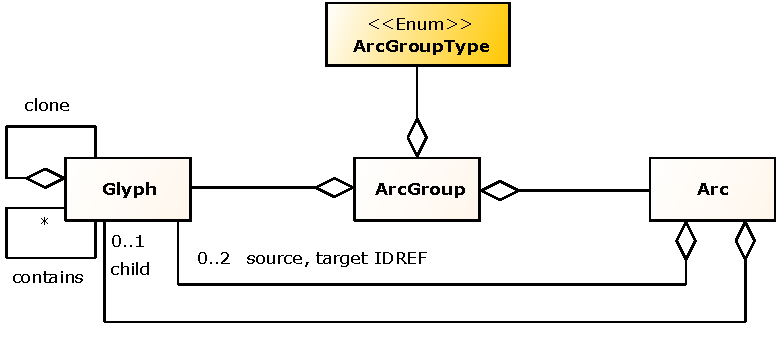
\includegraphics[scale=1.0]{figures/sbgnml_arcgroup_uml.pdf}\\
\caption{A UML representation of the \ArcGroup class for the
\SbgnmlPackage. See \ref{conventions} for conventions related to this
figure. }
  \label{fig:sbgnml_arcgroup_uml}
\end{figure}


The arc group describes a set of arcs and glyphs that have a relation together, for example, in ER arcs of class \const{interaction} around a glyph of class \const{interaction}.

Note that, despite the name, an arc group contains both arcs and glyphs.


The \ArcGroup object derives from the \SbgnBase class and thus inherits all
attributes and elements that are present for this class.

An \ArcGroup can contain:

\begin{itemize}
  \item zero or more child \Glyph elements,
  \item zero or more child \Arc elements.
\end{itemize}

In addition, the \ArcGroup object has the following attributes.

\paragraph{The \fixttspace\token{class} attribute}

An \ArcGroup has a required attribute \token{class} of type
\primtype{string}. While the type is of \primtype{string}, the values should be one of the ones defined in \primtype{ArcGroupType}.

\paragraph{The \Glyph element of an \ArcGroup}
An \ArcGroup can contain \Glyph{}s. For example, an \ArcGroup of class \const{interaction} must contain one \Glyph of class \const{interaction} representing the circle of an $n$-ary interaction. The glyph itself can contain one or more child \Glyph{}s of the class \const{outcome}. Please note, the  specification for the Entity Relationship language does not define a \Glyph node of class \const{interaction}. It is only introduced here to represent the circle mentioned above.

\paragraph{The \Arc element of an \ArcGroup}
An \ArcGroup can have multiple \Arc{}s. They are all assumed to form a single hyperarc-like structure.

\paragraph{Example}

The following example shows an \ArcGroup definition within an abbreviated SBGN map definition. The example shows an \ArcGroup of class \const{interaction} with the \Glyph of class \const{interaction} and two \Arc{}s of class \const{interaction}. The glyph contains one child, a \Glyph of the class \const{outcome}. \ref{fig:arcgroup_example} shows the corresponding visual representation.

\begin{example}
<map ...>
    ...
    <arcgroup class="interaction">
        <glyph id="glyph1" class="interaction">
            <bbox x="180.0" y="17.5" w="35.0" h="35.0"/>
            <glyph id="glyph1a" class="outcome">
                <bbox x="191.5" y="46.5" w="12.0" h="12.0"/>
            </glyph>
        </glyph>
        <arc id="arc1" class="interaction" source="glyph1" target="glyph2">
            <start x="180.0" y="35.0"/>
            <end x="110.0" y="35.0"/>
        </arc>
        <arc id="arc2" class="interaction" source="glyph1" target="glyph3">
            <start x="215.0" y="35.0"/>
            <end x="285.0" y="35.0"/>
        </arc>
    </arcgroup>
    ...
</map>
\end{example}

\begin{figure}[!ht]
  \centering
  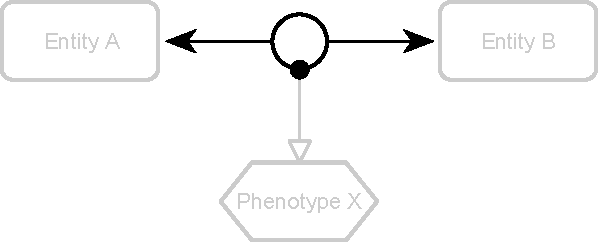
\includegraphics[scale=0.9]{figures/arcgroup_example_v2.pdf}
\caption{Visual representation of an \ArcGroup of class \const{interaction} with one \Glyph of class \const{interaction} and two \Arc{}s.}
  \label{fig:arcgroup_example}
\end{figure}


%-------------------------------------------------------------------
\section{Example SBGN Maps}
\label{examples}

This section provides complete examples, one for each SBGN language, showing how to use the elements described in the previous section, in sample SBGN maps.

\subsection{Example of a Process Description Map}

The following example of a Process Description map shows a gene-regulatory network -- the activated STAT1$\upalpha$ induction of the IRF1 gene. \ref{fig:pd_example} shows the corresponding visual representation of the Process Description map.

\begin{example}
<?xml version="1.0" encoding="UTF-8" standalone="yes"?>
<sbgn xmlns="http://sbgn.org/libsbgn/0.3">
    <map id="map1" language="process description">
        <glyph id="glyph0" class="complex">
            <bbox x="5.0" y="2.5" w="180.0" h="105.0"/>
            <glyph id="glyph1" class="macromolecule">
                <label text="STAT1$\alpha$"/>
                <bbox x="25.0" y="25.0" w="140.0" h="60.0"/>
                <glyph id="glyph1a" class="unit of information">
                    <label text="mt:prot"/>
                    <bbox x="36.0" y="16.5" w="48.0" h="17.0"/>
                </glyph>
            </glyph>
        </glyph>
        <glyph id="glyph2" class="nucleic acid feature">
            <label text="IRF1-GAS"/>
            <bbox x="235.0" y="25.0" w="120.0" h="60.0"/>
            <glyph id="glyph2a" class="unit of information">
                <label text="ct:grr"/>
                <bbox x="244.5" y="16.5" w="41.0" h="17.0"/>
            </glyph>
        </glyph>
        <glyph id="glyph3" class="nucleic acid feature">
            <label text="IRF1"/>
            <bbox x="465.0" y="430.0" w="120.0" h="60.0"/>
            <glyph id="glyph3a" class="unit of information">
                <label text="ct:mRNA"/>
                <bbox x="496.5" y="421.5" w="57.0" h="17.0"/>
            </glyph>
        </glyph>
        <glyph id="glyph4" class="and" orientation="vertical">
            <bbox x="375.0" y="365.0" w="40.0" h="40.0"/>
            <port id="glyph4.2" x="395.0" y="425.0"/>
            <port id="glyph4.1" x="395.0" y="345.0"/>
        </glyph>
        <glyph id="glyph5" class="process">
            <bbox x="515.0" y="540.0" w="20.0" h="20.0"/>
            <port id="glyph5.1" x="505.0" y="550.0"/>
            <port id="glyph5.2" x="545.0" y="550.0"/>
        </glyph>
        <glyph id="glyph6" class="process">
            <bbox x="385.0" y="450.0" w="20.0" h="20.0"/>
            <port id="glyph6.1" x="375.0" y="460.0"/>
            <port id="glyph6.2" x="415.0" y="460.0"/>
        </glyph>
        <glyph id="glyph7" class="source and sink">
            <bbox x="425.0" y="530.0" w="40.0" h="40.0"/>
        </glyph>
        <glyph id="glyph8" class="source and sink">
            <bbox x="295.0" y="440.0" w="40.0" h="40.0"/>
        </glyph>
        <glyph id="glyph9" class="association" orientation="vertical">
            <bbox x="165.0" y="150.0" w="20.0" h="20.0"/>
            <port id="glyph9.2" x="175.0" y="180.0"/>
            <port id="glyph9.1" x="175.0" y="140.0"/>
        </glyph>
        <glyph id="glyph13" class="complex">
            <bbox x="65.0" y="207.5" w="220.0" h="215.0"/>
            <glyph id="glyph11" class="complex">
                <bbox x="85.0" y="222.5" w="180.0" h="105.0"/>
                <glyph id="glyph10" class="macromolecule">
                    <label text="STAT1$\alpha$"/>
                    <bbox x="105.0" y="245.0" w="140.0" h="60.0"/>
                    <glyph id="glyph10a" class="unit of information">
                        <label text="mt:prot"/>
                        <bbox x="151.0" y="236.5" w="48.0" h="17.0"/>
                    </glyph>
                </glyph>
            </glyph>
            <glyph id="glyph12" class="nucleic acid feature">
                <label text="IRF1-GAS"/>
                <bbox x="115.0" y="350.0" w="120.0" h="60.0"/>
                <glyph id="glyph12a" class="unit of information">
                    <label text="ct:grr"/>
                    <bbox x="154.5" y="341.5" w="41.0" h="17.0"/>
                </glyph>
            </glyph>
        </glyph>
        <glyph id="glyph14" class="nucleic acid feature">
            <label text="IRF1"/>
            <bbox x="455.0" y="275.0" w="120.0" h="60.0"/>
            <glyph id="glyph14a" class="unit of information">
                <label text="ct:gene"/>
                <bbox x="489.5" y="266.5" w="51.0" h="17.0"/>
            </glyph>
        </glyph>
        <glyph id="glyph15" class="macromolecule">
            <label text="IRF1"/>
            <bbox x="590.0" y="520.0" w="120.0" h="60.0"/>
            <glyph id="glyph15a" class="unit of information">
                <label text="mt:prot"/>
                <bbox x="626.0" y="511.5" w="48.0" h="17.0"/>
            </glyph>
        </glyph>
        <arc id="arc0" class="necessary stimulation" source="glyph4.2" target="glyph6">
            <start x="395.0" y="425.0"/>
            <end x="395.0" y="450.0"/>
        </arc>
        <arc id="arc1" class="necessary stimulation" source="glyph3" target="glyph5">
            <start x="525.0" y="490.0"/>
            <end x="525.0" y="540.0"/>
        </arc>
        <arc id="arc2" class="consumption" source="glyph8" target="glyph6.1">
            <start x="335.0" y="460.0"/>
            <end x="375.0" y="460.0"/>
        </arc>
        <arc id="arc3" class="production" source="glyph6.2" target="glyph3">
            <start x="415.0" y="460.0"/>
            <end x="465.0" y="460.0"/>
        </arc>
        <arc id="arc4" class="consumption" source="glyph7" target="glyph5.1">
            <start x="465.0" y="550.0"/>
            <end x="505.0" y="550.0"/>
        </arc>
        <arc id="arc5" class="production" source="glyph5.2" target="glyph15">
            <start x="545.0" y="550.0"/>
            <end x="590.0" y="550.0"/>
        </arc>
        <arc id="arc6" class="production" source="glyph9.2" target="glyph13">
            <start x="175.0" y="180.0"/>
            <end x="175.0" y="207.5"/>
        </arc>
        <arc id="arc7" class="logic arc" source="glyph14" target="glyph4.1">
            <start x="455.0" y="325.0"/>
            <end x="395.0" y="345.0"/>
        </arc>
        <arc id="arc8" class="logic arc" source="glyph13" target="glyph4.1">
            <start x="285.0" y="330.0"/>
            <end x="395.0" y="345.0"/>
        </arc>
        <arc id="arc9" class="consumption" source="glyph0" target="glyph9.1">
            <start x="144.5" y="107.5"/>
            <end x="175.0" y="140.0"/>
        </arc>
        <arc id="arc10" class="consumption" source="glyph2" target="glyph9.1">
            <start x="252.5" y="85.0"/>
            <end x="175.0" y="140.0"/>
        </arc>
    </map>
</sbgn>
\end{example}

\begin{figure}[!ht]
  \centering
  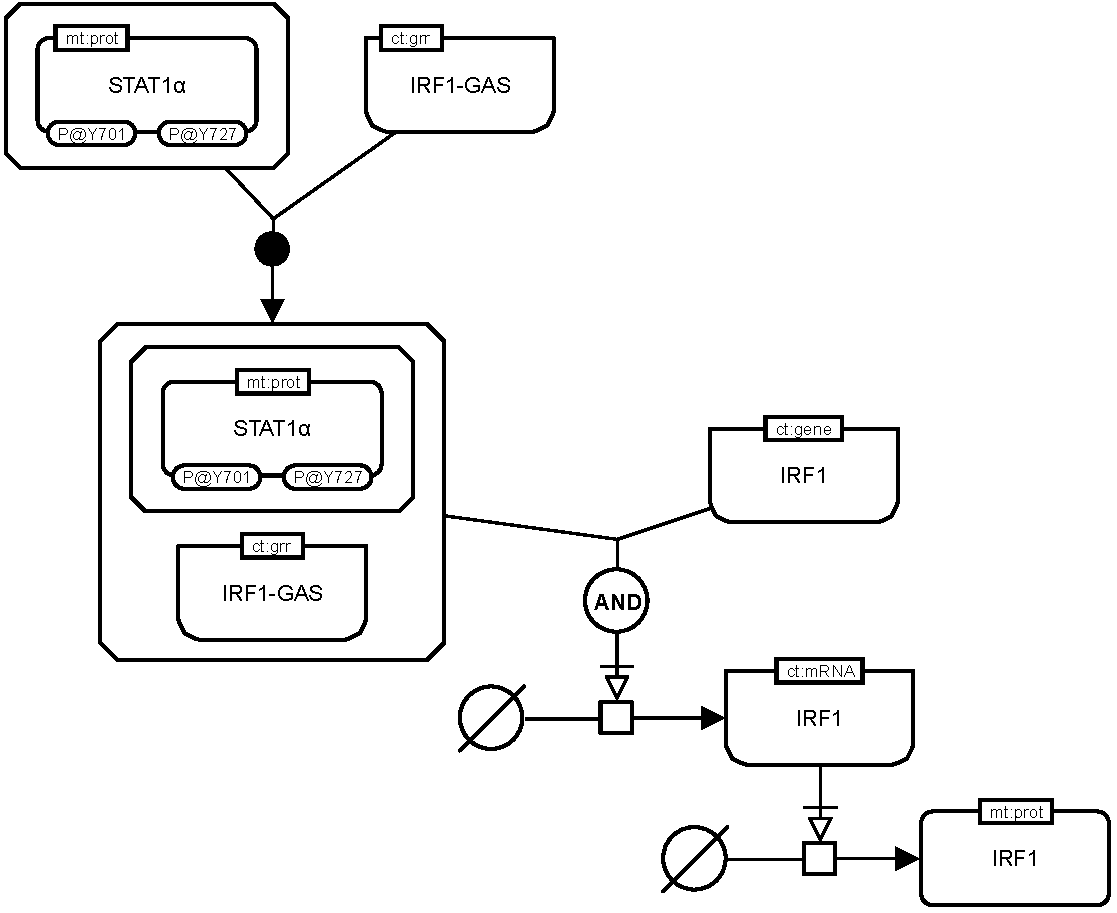
\includegraphics[scale=0.69]{figures/pd_example.pdf}
\caption{Activated STAT1$\alpha$ induction of the IRF1 gene.}
  \label{fig:pd_example}
\end{figure}

\clearpage

\subsection{Example of an Entity Relationship Map}

The following example of an Entity Relationship map shows the principle of the Polymerase Chain Reaction (PCR) \citep{Mullis1986}. \ref{fig:er_example} shows the corresponding visual representation of the Entity Relationship map.

\begin{example}
<?xml version="1.0" encoding="UTF-8" standalone="yes"?>
<sbgn xmlns="http://sbgn.org/libsbgn/0.3">
    <map id="map1" language="entity relationship">
        <glyph id="glyph0" class="entity">
            <label text="5' primer"/>
            <bbox x="361.0" y="435.0" w="108.0" h="60.0"/>
            <glyph id="glyph0a" class="unit of information">
                <label text="mt:dna"/>
                <bbox x="391.0" y="487.0" w="48.0" h="16.0"/>
            </glyph>
        </glyph>
        <glyph id="glyph1" class="entity">
            <label text="Antisense"/>
            <bbox x="361.0" y="135.0" w="108.0" h="60.0"/>
            <glyph id="glyph1a" class="unit of information">
                <label text="mt:dna"/>
                <bbox x="391.0" y="127.0" w="48.0" h="16.0"/>
            </glyph>
            <glyph id="glyph1b" class="existence">
                <bbox x="377.0" y="182.5" w="22.0" h="25.0"/>
            </glyph>
        </glyph>
        <glyph id="glyph2" class="entity">
            <label text="3' primer"/>
            <bbox x="61.0" y="435.0" w="108.0" h="60.0"/>
            <glyph id="glyph2a" class="unit of information">
                <label text="mt:dna"/>
                <bbox x="91.0" y="487.0" w="48.0" h="16.0"/>
            </glyph>
        </glyph>
        <glyph id="glyph3" class="entity">
            <label text="Sense"/>
            <bbox x="61.0" y="135.0" w="108.0" h="60.0"/>
            <glyph id="glyph3a" class="unit of information">
                <label text="mt:dna"/>
                <bbox x="91.0" y="127.0" w="48.0" h="16.0"/>
            </glyph>
            <glyph id="glyph3b" class="existence">
                <bbox x="131.0" y="182.5" w="22.0" h="25.0"/>
            </glyph>
        </glyph>
        <glyph id="glyph4" class="perturbing agent">
            <label text="Heat"/>
            <bbox x="211.0" y="5.0" w="108.0" h="60.0"/>
        </glyph>
        <glyph id="glyph5" class="or" orientation="vertical">
            <bbox x="244.0" y="271.0" w="42.0" h="42.0"/>
            <port id="glyph5.1" x="265.0" y="250.0"/>
            <port id="glyph5.2" x="265.0" y="334.0"/>
        </glyph>
        <glyph id="glyph6" class="variable value">
            <label text="T"/>
            <bbox x="378.0" y="275.0" w="20.0" h="20.0"/>
        </glyph>
        <glyph id="glyph7" class="variable value">
            <label text="T"/>
            <bbox x="132.0" y="275.0" w="20.0" h="20.0"/>
        </glyph>
        <arc id="arc0" class="interaction" source="glyph3" target="glyph1">
            <glyph id="arc0.0" class="outcome">
                <bbox x="219.0" y="159.0" w="12.0" h="12.0"/>
            </glyph>
            <port id="arc0.1" x="265.0" y="165.0"/>
            <glyph id="arc0.2" class="outcome">
                <bbox x="299.0" y="159.0" w="12.0" h="12.0"/>
            </glyph>
            <start x="169.0" y="165.0"/>
            <end x="361.0" y="165.0"/>
        </arc>
        <arc id="arc1" class="interaction" source="glyph2" target="glyph3">
            <glyph id="arc1.0" class="outcome">
                <bbox x="109.0" y="379.0" w="12.0" h="12.0"/>
            </glyph>
            <glyph id="arc1.1" class="outcome">
                <bbox x="109.0" y="329.0" w="12.0" h="12.0"/>
            </glyph>
            <port id="arc1.2" x="115.0" y="285.0"/>
            <port id="arc1.3" x="115.0" y="245.0"/>
            <start x="115.0" y="435.0"/>
            <end x="115.0" y="195.0"/>
        </arc>
        <arc id="arc2" class="interaction" source="glyph0" target="glyph1">
            <glyph id="arc2.0" class="outcome">
                <bbox x="409.0" y="359.0" w="12.0" h="12.0"/>
            </glyph>
            <glyph id="arc2.1" class="outcome">
                <bbox x="409.0" y="329.0" w="12.0" h="12.0"/>
            </glyph>
            <port id="arc2.2" x="415.0" y="285.0"/>
            <port id="arc2.3" x="415.0" y="245.0"/>
            <start x="415.0" y="435.0"/>
            <end x="415.0" y="195.0"/>
        </arc>
        <arc id="arc3" class="assignment" source="glyph7" target="glyph3">
            <port id="arc3.0" x="142.0" y="245.0"/>
            <start x="139.75" y="275.0"/>
            <end x="142.0" y="200.0"/>
        </arc>
        <arc id="arc4" class="assignment" source="glyph6" target="glyph1">
            <port id="arc4.0" x="388.0" y="245.0"/>
            <start x="390.25" y="275.0"/>
            <end x="388.0" y="200.0"/>
        </arc>
        <arc id="arc5" class="absolute inhibition" source="glyph4" target="arc0.1">
            <start x="265.0" y="65.0"/>
            <end x="265.0" y="165.0"/>
        </arc>
        <arc id="arc6" class="absolute inhibition" source="glyph5.1" target="arc0.1">
            <start x="265.0" y="250.0"/>
            <end x="265.0" y="165.0"/>
        </arc>
        <arc id="arc7" class="absolute inhibition" source="glyph4" target="arc2.2">
            <start x="273.4" y="65.0"/>
            <next x="279.0" y="85.0"/>
            <next x="525.0" y="85.0"/>
            <next x="525.0" y="285.0"/>
            <end x="415.0" y="285.0"/>
        </arc>
        <arc id="arc8" class="absolute inhibition" source="arc0.2" target="arc2.3">
            <start x="305.0" y="159.0"/>
            <next x="305.0" y="95.0"/>
            <next x="515.0" y="95.0"/>
            <next x="515.0" y="245.0"/>
            <end x="415.0" y="245.0"/>
        </arc>
        <arc id="arc9" class="necessary stimulation" source="arc2.0" target="arc3.0">
            <start x="409.0" y="365.0"/>
            <next x="185.0" y="365.0"/>
            <next x="185.0" y="245.0"/>
            <end x="142.0" y="245.0"/>
        </arc>
        <arc id="arc10" class="necessary stimulation" source="arc1.0" target="arc4.0">
            <start x="121.0" y="385.0"/>
            <next x="345.0" y="385.0"/>
            <next x="345.0" y="245.0"/>
            <end x="388.0" y="245.0"/>
        </arc>
        <arc id="arc11" class="absolute inhibition" source="glyph4" target="arc1.2">
            <start x="256.6" y="65.0"/>
            <next x="251.0" y="85.0"/>
            <next x="5.0" y="85.0"/>
            <next x="5.0" y="285.0"/>
            <end x="115.0" y="285.0"/>
        </arc>
        <arc id="arc12" class="absolute inhibition" source="arc0.0" target="arc1.3">
            <start x="225.0" y="159.0"/>
            <next x="225.0" y="95.0"/>
            <next x="15.0" y="95.0"/>
            <next x="15.0" y="245.0"/>
            <end x="115.0" y="245.0"/>
        </arc>
        <arc id="arc13" class="logic arc" source="arc1.1" target="glyph5.2">
            <start x="121.0" y="335.0"/>
            <end x="265.0" y="334.0"/>
        </arc>
        <arc id="arc14" class="logic arc" source="arc2.1" target="glyph5.2">
            <start x="409.0" y="335.0"/>
            <end x="265.0" y="334.0"/>
        </arc>
    </map>
</sbgn>
\end{example}

\begin{figure}[!ht]
  \centering
  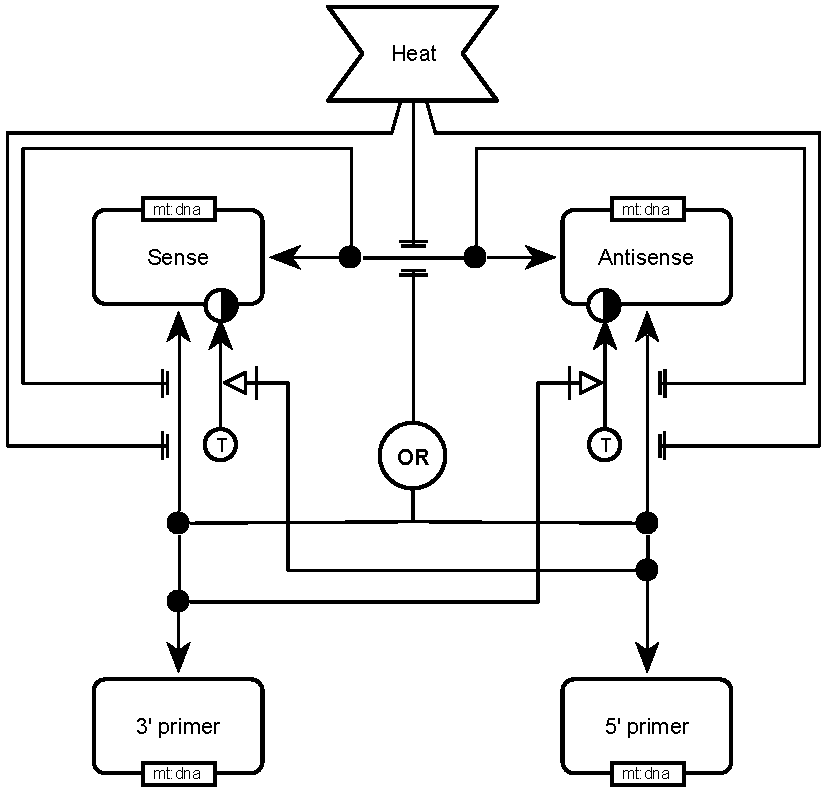
\includegraphics[scale=0.69]{figures/er_example.pdf}
\caption{Principle of the Polymerase Chain Reaction (PCR) \citep{Mullis1986}.}
  \label{fig:er_example}
\end{figure}
\clearpage

\subsection{Example of an Activity Flow Map}

The following example of an Activity Flow map shows a signaling pathway involving the regulation of TGF$\upbeta$-induced metastasis, as described by \citet{Adorno2009}. \ref{fig:af_example} shows the corresponding visual representation of the Activity Flow map.

\begin{example}
<?xml version="1.0" encoding="UTF-8" standalone="yes"?>
<sbgn xmlns="http://sbgn.org/libsbgn/0.3">
    <map id="map1" language="activity flow">
        <glyph id="glyph0" class="phenotype">
            <label text="Pro-invasion&#xA;migration&#xA;metastasis&#xA;gene expression&#xA;platform"/>
            <bbox x="235.0" y="187.5" w="130.0" h="75.0"/>
        </glyph>
        <glyph id="glyph1" class="biological activity">
            <label text="Metastatic&#xA;suppressor&#xA;genes&#xA;activity"/>
            <bbox x="246.0" y="380.0" w="108.0" h="60.0"/>
        </glyph>
        <glyph id="glyph2" class="biological activity">
            <label text="TGF beta"/>
            <bbox x="246.0" y="5.0" w="108.0" h="60.0"/>
        </glyph>
        <glyph id="glyph3" class="biological activity">
            <label text="Mutant p53/&#xA;P-Smad"/>
            <bbox x="6.0" y="205.0" w="108.0" h="60.0"/>
        </glyph>
        <glyph id="glyph4" class="biological activity">
            <label text="p63"/>
            <bbox x="6.0" y="380.0" w="108.0" h="60.0"/>
        </glyph>
        <glyph id="glyph5" class="biological activity">
            <label text="Ras"/>
            <bbox x="4.0" y="5.0" w="72.0" h="40.0"/>
        </glyph>
        <glyph id="glyph6" class="and" orientation="vertical">
            <bbox x="39.0" y="124.0" w="42.0" h="42.0"/>
            <port id="glyph6.1" x="60.0" y="103.0"/>
            <port id="glyph6.2" x="60.0" y="187.0"/>
        </glyph>
        <arc id="arc0" class="positive influence" source="glyph2" target="glyph0">
            <start x="300.0" y="65.0"/>
            <end x="300.0" y="187.5"/>
        </arc>
        <arc id="arc1" class="positive influence" source="glyph6.2" target="glyph3">
            <start x="60.0" y="187.0"/>
            <end x="60.0" y="205.0"/>
        </arc>
        <arc id="arc2" class="necessary stimulation" source="glyph4" target="glyph1">
            <start x="114.0" y="410.0"/>
            <end x="246.0" y="410.0"/>
        </arc>
        <arc id="arc3" class="logic arc" source="glyph5" target="glyph6.1">
            <start x="45.0" y="45.0"/>
            <end x="60.0" y="103.0"/>
        </arc>
        <arc id="arc4" class="negative influence" source="glyph3" target="glyph4">
            <start x="60.0" y="265.0"/>
            <end x="60.0" y="380.0"/>
        </arc>
        <arc id="arc5" class="negative influence" source="glyph1" target="glyph0">
            <start x="300.0" y="380.0"/>
            <end x="300.0" y="262.5"/>
        </arc>
        <arc id="arc6" class="logic arc" source="glyph2" target="glyph6.1">
            <start x="246.0" y="35.0"/>
            <next x="160.0" y="35.0"/>
            <end x="60.0" y="103.0"/>
        </arc>
    </map>
</sbgn>
\end{example}

\begin{figure}[!ht]
  \centering
  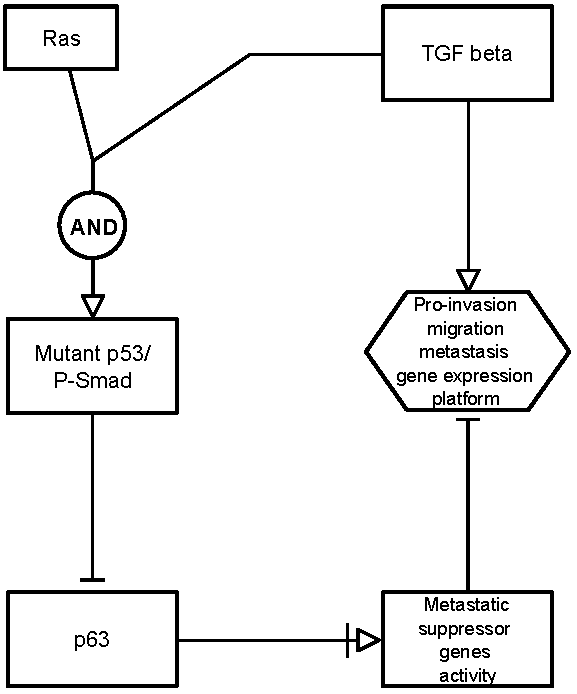
\includegraphics[scale=0.69]{figures/af_example.pdf}
\caption{Regulation of TGF$\beta$--induced metastasis as described by \citet{Adorno2009}.}
  \label{fig:af_example}
\end{figure}
